\documentclass[aspectratio=169]{beamer}

\usetheme{Madrid}
\usecolortheme{dolphin}
\setbeamertemplate{navigation symbols}{}

\usepackage{amsmath,amssymb}
\usepackage{graphicx}
\usepackage{booktabs}
\usepackage{tikz}
\usetikzlibrary{arrows.meta, positioning}

% Speaker notes
\usepackage{pgfpages}
% Uncomment one of these depending on how you want notes
%\setbeameroption{show notes} % show notes under slides
%\setbeameroption{show notes on second screen=right}

\title{A Dual--SPMA Framework for Convex MDPs}
\subtitle{Fenchel Duality + Softmax Policy Mirror Ascent}
\author{Shervin Khamooshian \and Ahmed Magd \and Pegah Aryadoost \and Danielle Nguyen}
\institute{School of Computing Science, Simon Fraser University}
\date{Project Presentation}

\begin{document}

%------------------------------------------------------------
\begin{frame}
  \titlepage
  \note{
    \begin{itemize}
      \item Welcome and introduce the project title.
      \item One-sentence claim: ``Fenchel duality plus a fast policy optimizer (SPMA) gives a simple way to solve convex MDPs; we compare this Dual--SPMA recipe against a CMDP baseline.''
      \item Briefly mention group members and that each of you will handle different sections.
    \end{itemize}
  }
\end{frame}

%------------------------------------------------------------
\begin{frame}{Outline}
  \tableofcontents
  \note{
    \begin{itemize}
      \item Walk through the outline:
      \item First: background and motivation.
      \item Second: formal convex MDP formulation and Fenchel dual.
      \item Third: related work: convex MDPs, SPMA, NPG--PD.
      \item Fourth: our Dual--SPMA method and implementation.
      \item Finally: experiments, conclusions, and future work.
    \end{itemize}
  }
\end{frame}

\section{Motivation \& Background}

%------------------------------------------------------------
\begin{frame}{What is an MDP?}
  \begin{itemize}
    \item Agent interacts with environment over time:
      \begin{itemize}
        \item Observe state $s_t$
        \item Choose action $a_t \sim \pi(\cdot|s_t)$
        \item Environment transitions to $s_{t+1}$, emits reward $r_t$
      \end{itemize}
    \item Policy $\pi$: mapping from states to action distributions.
    \item Goal: do well in the long run.
  \end{itemize}

  \vspace{0.3cm}
  \begin{center}
    % Placeholder for cartoon loop
    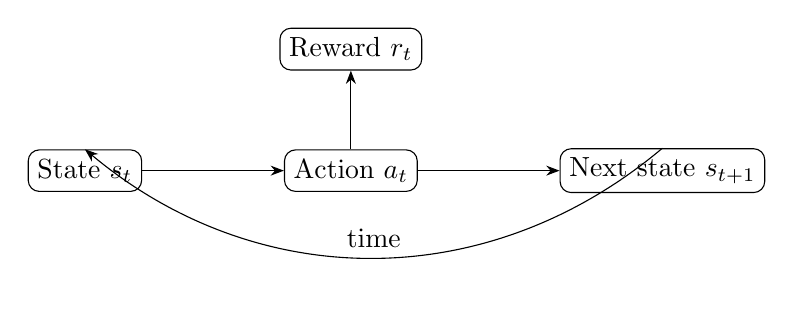
\begin{tikzpicture}[node distance=1.8cm, >=Stealth]
      \node[draw, rounded corners] (s) {State $s_t$};
      \node[draw, rounded corners, right=of s] (a) {Action $a_t$};
      \node[draw, rounded corners, right=of a] (sp) {Next state $s_{t+1}$};
      \node[draw, rounded corners, above=1cm of a] (r) {Reward $r_t$};

      \draw[->] (s) -- (a);
      \draw[->] (a) -- (sp);
      \draw[->] (a) -- (r);
      \draw[->, bend left=40] (sp.north) to node[above]{time} (s.north);
    \end{tikzpicture}
  \end{center}

  \note{
    \begin{itemize}
      \item Give a simple, intuitive description of the RL loop.
      \item Emphasize that the policy can be stochastic.
      \item We care about long-run performance, not just immediate rewards.
    \end{itemize}
  }
\end{frame}

%------------------------------------------------------------
\begin{frame}{Standard RL objective}
  \begin{itemize}
    \item Discounted return:
      \[
      J(\pi) = (1-\gamma)\,\mathbb{E}\Big[ \sum_{t=0}^{\infty} \gamma^t r(s_t,a_t) \Big]
      \]
    \item RL aims to find $\pi^\star = \arg\max_\pi J(\pi)$.
    \item We will re-express this in terms of \emph{where} the policy spends time.
  \end{itemize}

  \note{
    \begin{itemize}
      \item Introduce the discounted return formula.
      \item Interpret $(1-\gamma)$ as a normalization factor.
      \item Motivate the idea of ``where the policy spends time'' as a bridge to occupancy measures.
    \end{itemize}
  }
\end{frame}

%------------------------------------------------------------
\begin{frame}{Occupancy measure: where the policy spends time}
  \begin{itemize}
    \item \textbf{Discounted occupancy measure:}
    \[
    d_\pi(s,a) = (1-\gamma)\sum_{t=0}^\infty \gamma^t \Pr_\pi(s_t=s,a_t=a)
    \]
    \item Think of $d_\pi$ as a heatmap over $(s,a)$:
      \begin{itemize}
        \item High where the policy visits often.
        \item Low where it rarely goes.
      \end{itemize}
    \item $d_\pi$ is a probability distribution over $(s,a)$.
  \end{itemize}

  \vspace{0.3cm}
  \begin{center}
    \includegraphics[width=0.55\textwidth]{figures/occupancy_heatmap.pdf}
  \end{center}

  \note{
    \begin{itemize}
      \item Define $d_\pi$ formally.
      \item Use the heatmap figure to give intuition.
      \item Point out that $\sum_{s,a} d_\pi(s,a) = 1$.
    \end{itemize}
  }
\end{frame}

%------------------------------------------------------------
\begin{frame}{RL is linear in occupancy}
  \begin{itemize}
    \item We can rewrite the return as:
      \[
      J(\pi) = \sum_{s,a} r(s,a) d_\pi(s,a) = \langle r, d_\pi \rangle
      \]
    \item Standard RL $\Rightarrow$ maximize a \textbf{linear} function of $d_\pi$.
    \item But many interesting goals are not linear in $d_\pi$:
      \begin{itemize}
        \item Safety constraints.
        \item Imitation (matching an expert occupancy).
        \item Exploration / entropy bonuses.
      \end{itemize}
  \end{itemize}

  \note{
    \begin{itemize}
      \item Emphasize the key identity $J(\pi)=\langle r,d_\pi\rangle$.
      \item Transition to the idea that we want more general convex functions of $d_\pi$.
      \item Mention examples: CMDPs, imitation learning, max-entropy RL.
    \end{itemize}
  }
\end{frame}

\section{Problem Formulation: Convex MDPs}

%------------------------------------------------------------
\begin{frame}{Convex MDPs}
  \begin{itemize}
    \item Let $D$ be the set of feasible occupancies (flow constraints).
    \item \textbf{Convex MDP:}
      \[
      \min_{\pi} f(d_\pi) \quad \Leftrightarrow \quad \min_{d\in D} f(d)
      \]
    \item Examples of $f(d)$ (Appendix A):
      \begin{itemize}
        \item \textbf{Constrained safety:} $f(d) = -\langle r,d\rangle + \lambda \max\{0,\langle c,d\rangle - \tau\}$.
        \item \textbf{Entropy-regularized RL:} $f(d) = -\langle r, d\rangle - \alpha H(\pi_d)$.
      \end{itemize}
  \end{itemize}

  \note{
    \begin{itemize}
      \item Define convex MDPs as minimizing a convex functional of $d_\pi$.
      \item Mention that standard RL is recovered when $f(d)=-\langle r,d\rangle$.
      \item Briefly remind the audience of the constrained safety and entropy examples from the proposal.
    \end{itemize}
  }
\end{frame}

%------------------------------------------------------------
\begin{frame}{Fenchel duality and saddle-point form}
  \begin{itemize}
    \item Fenchel conjugate: $f^\ast(y) = \sup_{x\in D} \{\langle y,x\rangle - f(x)\}$.
    \item Fenchel--Moreau:
      \[
      f(d) = \max_{y} \{\langle y,d\rangle - f^\ast(y)\}
      \]
    \item Plug into the convex MDP:
      \[
      \min_{d\in D} f(d) = \min_{d\in D} \max_{y} \{\langle y,d\rangle - f^\ast(y)\}
      \]
      \[
      = \min_{\pi} \max_{y} L(\pi,y),\quad L(\pi,y)=\langle y,d_\pi\rangle - f^\ast(y)
      \]
  \end{itemize}

  \note{
    \begin{itemize}
      \item Introduce the Fenchel conjugate and the Fenchel--Moreau identity.
      \item Explain that this gives us a min--max (saddle-point) formulation.
      \item Emphasize that now we can think of two ``players'': policy and dual.
    \end{itemize}
  }
\end{frame}

%------------------------------------------------------------
\begin{frame}{From convex objective to shaped reward}
  \begin{itemize}
    \item For fixed $y$, minimizing $L(\pi,y)$ over $\pi$ is equivalent to:
      \[
      \min_{\pi} \langle y, d_\pi \rangle
      \]
    \item Using the discounted occupancy identity:
      \[
      \langle y, d_\pi \rangle
      = (1-\gamma)\,\mathbb{E}_\pi\Big[ \sum_{t\ge0} \gamma^t y(s_t,a_t) \Big]
      \]
    \item So the policy step is standard RL with shaped reward:
      \[
      r_y(s,a) = -y(s,a)
      \]
      (or $r_y(s,a) = -\phi(s,a)^\top w$ in FA).
  \end{itemize}

  \note{
    \begin{itemize}
      \item Show how $\langle y,d_\pi\rangle$ becomes a discounted return.
      \item Conclude that for fixed $y$, the policy player just sees a shaped reward $r_y$.
      \item This motivates our design: we can plug any RL algorithm as the policy player.
    \end{itemize}
  }
\end{frame}

\section{Related Work}

%------------------------------------------------------------
\begin{frame}{Related work: convex MDPs and general utilities}
  \begin{itemize}
    \item \textbf{Convex MDPs} (Zahavy et al., 2021):
      \begin{itemize}
        \item Formalize convex MDPs and the Fenchel dual reduction.
        \item Provide a meta-algorithm with policy and cost players.
      \end{itemize}
    \item \textbf{General utilities / occupancy methods}:
      \begin{itemize}
        \item Recent work characterizes policy gradient methods on utility functions of occupancies.
        \item Highlights importance of efficient occupancy estimation in large spaces.
      \end{itemize}
  \end{itemize}

  \note{
    \begin{itemize}
      \item Briefly mention Zahavy et al.'s contribution: convex MDP framework + meta-algorithm.
      \item Mention general utilities line (Barakat et al., etc.) which looks at global optimality in the occupancy space.
      \item Position our work as a concrete instantiation of this general picture.
    \end{itemize}
  }
\end{frame}

%------------------------------------------------------------
\begin{frame}{Related work: SPMA and policy-gradient geometry}
  \begin{itemize}
    \item Trust-region and mirror-descent methods:
      \begin{itemize}
        \item TRPO, PPO, MDPO: geometry-aware PG with KL or mirror maps.
      \end{itemize}
    \item \textbf{Softmax Policy Mirror Ascent (SPMA)} (Asad et al., 2024):
      \begin{itemize}
        \item Mirror ascent in the \emph{logit space} using log-sum-exp mirror map.
        \item Tabular update:
          \[
          \pi_{t+1}(a|s) = \pi_t(a|s)\big(1 + \eta A^{\pi_t}(s,a)\big)
          \]
        \item Linear convergence in tabular MDPs, convex projection in FA.
      \end{itemize}
  \end{itemize}

  \note{
    \begin{itemize}
      \item Explain SPMA at a high level: mirror ascent in logits rather than probabilities.
      \item Highlight why SPMA is attractive: fast convergence and clean FA story.
      \item This motivates choosing SPMA as our policy player.
    \end{itemize}
  }
\end{frame}

%------------------------------------------------------------
\begin{frame}{Related work: CMDP primal--dual methods (NPG--PD)}
  \begin{itemize}
    \item \textbf{NPG--PD} (Ding et al., 2020):
      \begin{itemize}
        \item Lagrangian: $L(\pi,\lambda) = V_r^\pi(\rho) + \lambda(V_g^\pi(\rho)-b)$.
        \item Updates:
          \begin{itemize}
            \item Natural policy gradient ascent on $\pi$.
            \item Projected subgradient ascent on $\lambda$.
          \end{itemize}
        \item Guarantees: $\mathcal{O}(1/\sqrt{T})$ gap and constraint violation, dimension-free.
      \end{itemize}
    \item Serves as our main CMDP baseline.
  \end{itemize}

  \note{
    \begin{itemize}
      \item Introduce NPG--PD as a state-of-the-art CMDP algorithm.
      \item Emphasize that we use it as a baseline for constrained safety experiments.
      \item Our Dual--SPMA method is a more general convex-MDP-based alternative.
    \end{itemize}
  }
\end{frame}

\section{Our Method: Dual--SPMA}

%------------------------------------------------------------

\begin{frame}{Baseline: NPG--PD in our setup}
\begin{itemize}
  \item CMDP Lagrangian (same as Dual--SPMA):
    \[
      L(\pi,\lambda) = J_r(\pi) + \lambda\,(J_c(\pi)-\tau).
    \]
  \item Primal step: one natural policy gradient step on the shaped reward
    \[
      r_\lambda(s,a) = r(s,a) - \lambda\,c(s,a),
    \]
    using a diagonal-Fisher NPG update on a softmax actor.
  \item Dual step: projected ascent on $\lambda$:
    \[
      \lambda_{k+1} = \big[\lambda_k + \beta\,(J_c(\pi_k) - \tau)\big]_+.
    \]
  \item Implementation mirrors Ding et al.\ (2020):
    \begin{itemize}
      \item Actor--critic with GAE advantages (same networks as SPMA).
      \item No shaped dual variables in the loss; only $r_\lambda$.
      \item One NPG step per outer iteration.
    \end{itemize}
\end{itemize}
\end{frame}

% "Now that we’ve looked at the theory of NPG‑PD, here’s how we actually implement it in our codebase.”
% “We keep the same Lagrangian as in the dual–SPMA CMDP formulation: reward plus a Lagrange multiplier times the constraint violation.”
% “The key difference is in the primal step. Instead of a mirror‑descent SPMA update, we do one natural policy gradient step on a shaped reward r_λ(s,a)=r(s,a)−λc(s,a)
% “The dual step is a projected gradient ascent on λ; when the expected cost exceeds τ we push λ up, otherwise it drifts down to zero.”
% “Implementation‑wise, we reuse our actor–critic architecture and GAE advantages. The only new piece is a diagonal‑Fisher natural gradient update, which approximates the NPG direction without computing a full Fisher matrix.

%------------------------------------------------------------
\begin{frame}{Dual--SPMA loop: high-level view}
  \begin{columns}
    \column{0.52\textwidth}
      \begin{itemize}
        \item We consider the saddle problem:
          \[
          \min_\pi \max_y L(\pi,y) = \langle y,d_\pi\rangle - f^\ast(y)
          \]
        \item \textbf{Outer loop (dual):} mirror ascent on $y$:
          \[
          y_{k+1} = y_k + \alpha (d_{\pi_k} - \nabla f^\ast(y_k))
          \]
        \item \textbf{Inner loop (policy):} run $K_{\text{in}}$ SPMA steps under reward $r_{y_k}$.
      \end{itemize}
    \column{0.45\textwidth}
      \begin{center}
        \includegraphics[width=\textwidth]{figures/dual_spma_diagram.pdf}
      \end{center}
  \end{columns}

  \note{
    \begin{itemize}
      \item Describe the two players: dual (cost) and policy.
      \item Explain that the dual step uses estimated occupancies, while the policy step solves a shaped RL problem.
      \item Point to the diagram showing the feedback loop: $y$ $\rightarrow$ shaped reward $\rightarrow$ policy $\rightarrow$ occupancy $\rightarrow$ dual update.
    \end{itemize}
  }
\end{frame}

%------------------------------------------------------------
\begin{frame}{Policy player: SPMA actor--critic oracle}
  \begin{itemize}
    \item Inner loop implemented as SPMA actor--critic:
      \begin{itemize}
        \item Softmax or Gaussian policy networks.
        \item Value critic + GAE advantages.
        \item SPMA loss on a batch:
          \[
          \mathcal{L} = \mathbb{E}\big[-\Delta\log\pi \cdot A
            + \frac{1}{\eta}\big(\exp(\Delta\log\pi)-1-\Delta\log\pi\big)\big]
          \]
      \end{itemize}
    \item We use Armijo backtracking (plus fallback) to choose the step size.
    \item Our \texttt{PolicyOracleSPMA} wraps:
      \begin{itemize}
        \item A shaped-reward env ($r_y=-y$ or $-\phi^\top w$).
        \item SPMA updates for $K_{\text{in}}$ iterations.
        \item Occupancy / feature estimators.
      \end{itemize}
  \end{itemize}

  \note{
    \begin{itemize}
      \item Explain that we implement SPMA as a loss in logit space, matching the theory.
      \item Mention that we use GAE and a critic, similar to PPO/TRPO.
      \item Clarify that the oracle takes a dual variable $y$, runs SPMA, and returns a policy snapshot plus occupancy estimates.
    \end{itemize}
  }
\end{frame}

%------------------------------------------------------------
\begin{frame}{Estimating occupancies and feature expectations}
  \begin{itemize}
    \item \textbf{Tabular estimator} (Appendix C):
      \[
      \hat d_\pi(s,a) = \frac{1-\gamma}{N}\sum_{i=1}^N \sum_t \gamma^t
        \mathbf{1}\{s_t^{(i)}=s,a_t^{(i)}=a\}
      \]
    \item \textbf{Feature estimator} (FA):
      \[
      \widehat{\mathbb{E}}[\phi] = \frac{1-\gamma}{N}\sum_{i,t}\gamma^t \phi(s_t^{(i)},a_t^{(i)})
      \]
    \item Both are implemented as simple Monte Carlo estimators with episode counting.
    \item We verified in tests that $\sum_{s,a} \hat d_\pi(s,a)\approx 1$.
  \end{itemize}

  \note{
    \begin{itemize}
      \item Highlight why occupancy estimation is needed: dual gradient $\nabla_y L = d_\pi - \nabla f^\ast(y)$.
      \item Show the formulas and mention they match the derivations in the proposal.
      \item Point out that in function approximation we only need inner products, not the full $d_\pi$ table.
    \end{itemize}
  }
\end{frame}

% “In the tabular setting, our Monte Carlo estimator is unbiased but its variance effectively grows with the number of features d, because we’re estimating each coordinate separately.”
% “Barakat et al. propose a different view: parametrize the normalized occupancy as a log‑linear density λ_ω(s,a) proportional to exp(ω^T φ(s,a)), and fit ω by maximum likelihood.”
% “The cool part is the theory: the ℓ1 error of this MLE scales with √(m/n), where m is the dimension of ω, and does not depend explicitly on the number of state–action pairs.”
% “We implement an MLE estimator exactly in this spirit: a small log‑linear model over state–action features trained with Adam on a weighted log‑likelihood, and we plug its normalized output back into the dual gradient.”

%------------------------------------------------------------
\begin{frame}{Occupancy estimation: MC vs MLE}
\begin{itemize}
  \item Current estimators (Appendix C):
    \begin{itemize}
      \item Tabular: discounted visit counts $ \hat d_\pi(s,a)$.
      \item FA: Monte Carlo estimate of $ \mathbb{E}_\pi[\phi(s,a)]$.
    \end{itemize}
    Variance scales with feature dimension $d$.
  \item MLE-style estimator (Barakat et al., 2024):
    \[
      \lambda_\omega(s,a) \propto \exp(\omega^\top \phi(s,a)).
    \]
    Fit $\omega$ by maximizing the (discounted) log-likelihood of $(s_t,a_t)$ samples.
  \item Guarantees: $\|\hat\lambda - \lambda_\pi\|_1 = O\big(\sqrt{m/n}\big)$,
        depends on parameter dimension $m$ instead of $|S||A|$.
  \item Implementation:
    \begin{itemize}
      \item Log-linear model over $(s,a)$ features.
      \item Adam updates on the weighted log-likelihood.
      \item Returns a normalized occupancy estimate $\hat d_\pi(s,a)$.
    \end{itemize}
\end{itemize}
\end{frame}


%------------------------------------------------------------
\begin{frame}{Outer loop: entropy-regularized RL example}
  \begin{itemize}
    \item Entropy-regularized objective (simplified occupancy form):
      \[
      f(d) = -\langle r,d\rangle + \alpha \sum_i d_i \log d_i
      \]
    \item Conjugate:
      \[
      f^\ast(y) = \alpha \log\sum_i \exp\big((y_i+r_i)/\alpha\big)
      \]
      \[
      \nabla f^\ast(y) = \mathrm{softmax}\big((y+r)/\alpha\big)
      \]
    \item Dual update:
      \[
      y_{k+1} = y_k + \alpha_y\big( \hat d_{\pi_k} - \mathrm{softmax}((y_k+r)/\alpha)\big)
      \]
    \item Policy step: SPMA under $r_{y_k}(s,a) = -y_k(s,a)$.
  \end{itemize}

  \note{
    \begin{itemize}
      \item Show how entropy regularization fits into our general template.
      \item Emphasize that the dual gradient has a closed form softmax, which is convenient.
      \item Clarify that $r$ here comes from the environment's original reward table.
    \end{itemize}
  }
\end{frame}

%------------------------------------------------------------
\begin{frame}{Outer loop: constrained safety via Lagrangian}
  \begin{itemize}
    \item CMDP: maximize $J_r(\pi)$ subject to $J_c(\pi)\le \tau$.
    \item Lagrangian:
      \[
      L(\pi,\lambda) = J_r(\pi) + \lambda(J_c(\pi)-\tau),\quad \lambda\ge 0
      \]
    \item Policy update:
      \[
      r_\lambda(s,a) = r(s,a) - \lambda c(s,a)
      \]
      implemented via $y_{\lambda}(s,a)=\lambda c(s,a)-r(s,a)$, $r_y=-y$.
    \item Dual update:
      \[
      \lambda_{k+1} = \big[\lambda_k + \beta (J_c(\pi_k)-\tau)\big]_+
      \]
  \end{itemize}

  \note{
    \begin{itemize}
      \item Explain that for constrained safety we use the classical Lagrangian dual instead of a complicated Fenchel conjugate.
      \item Show how SPMA simply plugs in as the policy optimizer under $r_\lambda$.
      \item Mention that this mirrors NPG--PD, but with SPMA instead of natural PG.
    \end{itemize}
  }
\end{frame}

\section{Experiments}

%------------------------------------------------------------
\begin{frame}{Experimental setup}
  \begin{itemize}
    \item \textbf{Environments:}
      \begin{itemize}
        \item FrozenLake (tabular) with deterministic transitions.
        \item Simple cost structure for constrained safety (unsafe states).
        \item Pendulum (FA) as a sanity check for feature expectations.
      \end{itemize}
    \item \textbf{Metrics:}
      \begin{itemize}
        \item Saddle objective $L(\pi,y)$ (when $f^\ast$ known).
        \item Constraint violation $J_c(\pi)-\tau$.
        \item $\sum d_\pi$ and $\|E[\phi]\|$ (estimator sanity).
        \item Average return under shaped reward.
      \end{itemize}
  \end{itemize}

  \note{
    \begin{itemize}
      \item Briefly describe the environments and why they were chosen.
      \item List the key metrics you'll show plots for.
      \item Mention that NPG--PD is the intended baseline for the CMDP experiments (if implemented).
    \end{itemize}
  }
\end{frame}

%------------------------------------------------------------
\begin{frame}{Results: Dual--SPMA outer loop (entropy example)}
  \begin{columns}
    \column{0.48\textwidth}
      \begin{center}
        \includegraphics[width=\textwidth]{figures/L_vs_iter_entropy.pdf}\\
        {\small $L(\pi,y)$ vs outer iterations}
      \end{center}
    \column{0.48\textwidth}
      \begin{center}
        \includegraphics[width=\textwidth]{figures/sum_d_vs_iter_entropy.pdf}\\
        {\small $\sum_{s,a} \hat d_\pi(s,a)$ vs iterations}
      \end{center}
  \end{columns}

  \note{
    \begin{itemize}
      \item Comment on how $L(\pi,y)$ evolves: does it stabilize, improve, oscillate?
      \item Show that $\sum d_\pi$ stays near 1, confirming the estimator.
      \item Mention any sensitivity you observed to the dual step size or SPMA inner steps.
    \end{itemize}
  }
\end{frame}

%------------------------------------------------------------
\begin{frame}{Results: constrained safety Dual--SPMA}
  \begin{columns}
    \column{0.48\textwidth}
      \begin{center}
        \includegraphics[width=\textwidth]{figures/Jr_Jc_vs_iter_cmdp.pdf}\\
        {\small $J_r(\pi_k)$ and $J_c(\pi_k)$ vs iterations}
      \end{center}
    \column{0.48\textwidth}
      \begin{center}
        \includegraphics[width=\textwidth]{figures/constraint_violation_vs_iter_cmdp.pdf}\\
        {\small $J_c(\pi_k)-\tau$ vs iterations and $\lambda_k$}
      \end{center}
  \end{columns}

  \note{
    \begin{itemize}
      \item Describe how reward and cost evolve as the dual $\lambda$ adjusts.
      \item Point out whether the constraint violation approaches zero.
      \item If you have NPG--PD curves, compare convergence and stability qualitatively.
    \end{itemize}
  }
\end{frame}

%------------------------------------------------------------

\begin{frame}{Results: Dual--SPMA vs NPG--PD (CMDP)}
\begin{columns}
\column{0.48\textwidth}
  \centering
  \includegraphics[width=\linewidth]{figures/Jr_vs_iter_spma_npg.pdf}\\
  {\small $J_r(\pi_k)$ vs outer iterations}
\column{0.48\textwidth}
  \centering
  \includegraphics[width=\linewidth]{figures/constraint_violation_vs_iter_spma_npg.pdf}\\
  {\small $J_c(\pi_k)-\tau$ and $\lambda_k$ vs iterations}
\end{columns}
\vspace{0.5em}
\begin{itemize}
  \item Both methods eventually satisfy the safety constraint.
  \item SPMA tends to take larger, geometry-aware steps; NPG--PD is smoother but needs tuning of the NPG step size.
  \item Constraint satisfaction behaviour mirrors the theory of NPG--PD.
\end{itemize}
\end{frame}



%------------------------------------------------------------
\begin{frame}{Results: occupancy heatmaps}
  \begin{center}
    \includegraphics[width=0.7\textwidth]{figures/occupancy_heatmaps_gridworld.pdf}
  \end{center}
  \begin{itemize}
    \item Heatmaps of $\hat d_\pi$ on a gridworld:
      \begin{itemize}
        \item Left: unconstrained / entropy-regularized policy.
        \item Right: constrained safety policy.
      \end{itemize}
  \end{itemize}

  \note{
    \begin{itemize}
      \item Use this slide to give an intuitive picture of how the policies differ.
      \item Point out that under safety constraints, the agent avoids certain cells.
      \item Under entropy regularization, occupancy is more spread out.
    \end{itemize}
  }
\end{frame}

\section{Conclusion \& Future Work}

%------------------------------------------------------------
\begin{frame}{Takeaways \& limitations}
  \begin{itemize}
    \item \textbf{Recipe:} convex MDP $\Rightarrow$ Fenchel dual $\Rightarrow$ shaped-reward RL + SPMA.
    \item SPMA provides a practical policy player with strong convergence properties in tabular and FA settings.
    \item We implemented:
      \begin{itemize}
        \item Dual--SPMA outer loops for entropy-regularized RL and constrained safety.
        \item A sample-based NPG--PD baseline on the same CMDP tasks.
        \item Three occupancy estimators: tabular MC, FA MC, and an MLE-style estimator.
      \end{itemize}
    \item Limitations:
      \begin{itemize}
        \item Experiments are still in low-dimensional environments.
        \item MLE estimator and FA dual loop not yet stress-tested on large continuous tasks.
      \end{itemize}
  \end{itemize}

  \note{
    \begin{itemize}
      \item Summarize the conceptual recipe and what you implemented.
      \item Be open about limitations to avoid overselling.
      \item Mention that these are stepping stones toward a full Dual--SPMA CMDP solver.
    \end{itemize}
  }
\end{frame}

%------------------------------------------------------------
\begin{frame}{Future work}
\begin{itemize}
  \item Extend NPG--PD vs Dual--SPMA comparison to larger CMDPs and function approximation.
  \item Study empirically how MLE-based occupancy estimation scales in high-dimensional FA.
  \item Explore more general convex objectives (risk, imitation) with the same dual--SPMA template.
  \item Investigate variance-reduction techniques for dual gradients in the FA setting.
\end{itemize}

  \note{
    \begin{itemize}
      \item Provide a concrete roadmap: more objectives, better occupancy estimation, stronger baselines.
      \item Tie back to the theoretical papers your supervisor suggested (e.g., global optimality, density features).
    \end{itemize}
  }
\end{frame}

%------------------------------------------------------------
\begin{frame}{Q\&A}
  \centering
  {\Huge Questions?}

  \note{
    \begin{itemize}
      \item Invite questions.
      \item Encourage comments on both theory and implementation details.
    \end{itemize}
  }
\end{frame}

\end{document}
